\documentclass[12pt]{article}

\usepackage[margin=1in]{geometry}
\usepackage{setspace}
\usepackage{footmisc}
\usepackage{hyperref}
\usepackage{titlesec}
\usepackage{graphicx}
\usepackage{tikz}
\usetikzlibrary{shapes.geometric, arrows.meta, positioning, fit}

\usepackage[backend=biber,style=apa]{biblatex}
\usepackage{newunicodechar}
\newunicodechar{−}{\textminus}

\addbibresource{references.bib}

% Set spacing
\onehalfspacing

% Title formatting
\titleformat{\section}{\normalfont\large\bfseries}{\thesection.}{1em}{}

% Author footnotes
\renewcommand{\thefootnote}{\fnsymbol{footnote}}

\title{\textbf{Agentic AI Against Aging Hackathon: Ovarian Aging Value Report}}
\author{
  Mark Kagach\footnote{Tilburg University, contact: \texttt{mark@markkagach.com}. We thank ...}
  \and
  Elias Schlie\footnote{Tilburg University, contact: \texttt{elias@eliasschlie.com}. }
}

\date{October 22, 2025}

\begin{document}

\maketitle
\newpage

\section{Executive Summary}
This report estimates the economic value of the therapeutic delay in menopause by 5 years. It was completed as part of the Agentic AI Against Aging Hackathon. First, we present an AI pipeline that collects, grades and extracts papers with their relevant metrics. Second, we document our economic methodology for estimating annual US direct and indirect costs. Third, we conclude the report by presenting the results.

The AI pipeline autonomously discovers and extracts risk metrics from research papers linking menopause timing to health outcomes across seven disease categories. Using a LangGraph-based state machine, the system iteratively generates PubMed queries, evaluates abstract relevance, downloads open-access PDFs, and extracts structured risk metrics (OR, HR, RR) with confidence intervals while assessing study quality via ROBIS criteria \parencite{whitingROBISNewTool2016}. The fully autonomous pipeline processed 1000+ papers and extracted 250+ high-quality risk metrics with complete metadata traceability. The complete source code is publicly available at \url{https://github.com/EliasSchlie/quantifying-the-value-of-delayed-ovarian-aging}.

In economic methodology we first calculate the net effect therapeutic menopause delay has on annual accidents per 100,000 women for several diseases (both positive and negative). Then we estimate the annual direct and indirect cost per accident for each disease. Lastly, we scale the results to US population to get the final estimate.
Due to the time and data constraints, the final cost is first and foremost a \textit{rough} estimate, we recommend considering it as a ±33\% range.

The results are as follows, ...


\newpage
\section{AI Pipeline}

\subsection{Overview and Motivation}
Systematic literature reviews require substantial manual effort: searching databases, screening hundreds of abstracts, downloading papers, extracting data tables, and assessing study quality. For our menopause timing research, we needed to collect risk metrics across seven disease categories from meta-analyses—a task that would traditionally require weeks of manual work by trained researchers.

We developed an autonomous AI agent to automate this entire pipeline, from query generation to structured data extraction. The system operates as a LangGraph state machine with nine nodes that iteratively discover relevant papers, evaluate their quality, and extract risk metrics with full metadata traceability. This approach enabled us to process 1000+ papers and extract 250+ metrics in a fraction of the time required for manual review, while maintaining rigorous quality standards through automated ROBIS assessment.

\subsection{Architecture}
The agent is implemented as a directed graph workflow with three types of nodes: AI-powered decision nodes, tool-based action nodes, and conditional routing nodes (see Appendix A for complete workflow diagram and routing logic). The workflow begins with query generation and terminates when either the target number of metrics is reached or search space is exhausted.

\textbf{AI-Powered Nodes:}
\begin{itemize}
    \item \texttt{create\_query}: Generates targeted PubMed search queries using domain knowledge, adapting based on previous attempts
    \item \texttt{check\_abstract}: Evaluates abstract relevance using LLM classification (relevant/not relevant)
    \item \texttt{extract\_metadata}: Extracts study metadata including sample size, geography, confounders, and number of included studies
    \item \texttt{evaluate\_robis}: Assesses study quality using the ROBIS framework, providing both categorical risk rating (Low/High/Unclear) and numerical validity score (0-10)
    \item \texttt{extract\_risk\_metrics}: Uses structured tool calls to extract odds ratios (OR), hazard ratios (HR), and relative risks (RR) with 95\% confidence intervals
\end{itemize}

\textbf{Tool and Logic Nodes:}
\begin{itemize}
    \item \texttt{search\_pubmed}: Queries PubMed E-utilities API for meta-analyses (up to 500 results per query)
    \item \texttt{filter\_papers}: Deduplicates papers based on DOIs of already-checked publications
    \item \texttt{download\_paper}: Downloads PDFs via DOI resolution with multiple fallback strategies, then converts to markdown
    \item \texttt{track\_failed\_download}: Logs paywalled papers to CSV for subsequent manual download and processing
\end{itemize}

The workflow incorporates four conditional routing points that determine next actions based on state (detailed in Appendix A, Table \ref{tab:routing}).

\subsection{Key Technical Components}

\textbf{PubMed Integration:} The system queries the NCBI E-utilities API with programmatically generated search strings that combine menopause timing terminology with disease-specific keywords. Queries are filtered to meta-analyses and systematic reviews only, and the agent learns from unsuccessful queries to reformulate searches.

\textbf{PDF Acquisition:} PDF downloads employ a multi-strategy approach: (1) direct arXiv access for preprints, (2) Unpaywall API queries for open-access versions, (3) Bright Data web unlocker for publisher sites, (4) direct DOI resolution, and (5) HTML-to-PDF conversion as a last resort. Failed downloads are logged with full metadata for manual processing.

\textbf{PDF-to-Markdown Conversion:} We developed a hybrid extraction pipeline combining Docling (for structural preservation and table extraction) with pymupdf4llm (for character encoding accuracy). The system identifies Unicode encoding errors in Docling output and corrects them using context-based matching with pymupdf's character-level extraction, preserving document structure while fixing encoding issues.

\textbf{Quality Assessment:} Each paper undergoes ROBIS (Risk Of Bias In Systematic reviews) evaluation \parencite{whitingROBISNewTool2016} via structured LLM prompts. The agent assesses four domains: study eligibility criteria, identification and selection of studies, data collection and study appraisal, and synthesis and findings. This produces both a categorical risk rating and a 0-10 numerical score, enabling downstream filtering by quality thresholds.

\textbf{Metric Extraction:} Risk metrics are extracted via LLM tool calls with strict validation: each metric must include menopause age thresholds (e.g., "<40 vs 50-55"), specific health outcome, metric type (OR/HR/RR), point estimate, and 95\% confidence interval. Vague age terms like "early menopause" are rejected to ensure precise age-risk mappings.

\subsection{Data Quality and Output}
The pipeline ran for multiple hours, outputting a CSV file, containing 250+ risk metrics spanning seven health outcomes: all-cause mortality, type 2 diabetes, cardiovascular disease, all-cause dementia, osteoporosis and fractures, breast cancer, and endometrial/ovarian cancer. Each record includes complete metadata: publication DOI, date, authors, sample size, number of included studies, geographic scope, adjusted confounders, ROBIS scores, and source traceability. This structured dataset enables systematic meta-analysis of menopause timing effects across diverse health outcomes while maintaining full provenance from extraction to analysis.

\newpage
\section{Economic Methodology}
\subsection{Disease Incidents}
Our target population is of all active scientists in the world that conduct research in the longevity field. Unfortunately, we are not aware of a field-wide dataset listing all active researchers. This poses a limitation we discuss later. Since we do not have a robust sampling frame, we use twofold non-probability sampling. First, we reach out to 1000 randomly selected researchers that have published in the last 1.5 years in 27 leading journals on aging that were selected by industry experts (see Appendix 1). Second, we use snowball sampling: we advertise the survey in social media, specifically in groups with longevity researchers we’d like to reach, and then we ask participants for further references.

\newpage
\section{Results}
\subsection{Respondents Overview}
We have reached out to 876 researchers personally via email in the period between May 2 and May 21 with 2 follow-ups. All together we got 64 completed surveys, excluding 17 pilot tested submissions, this is 47 final respondents.  The completion rate is 61\%, and average duration is 11 minutes 16 seconds. We cannot calculate the precise response rate as the survey is anonymous, and some have participated through email, but didn’t let us know. Yet, based on the social media engagement, and some data from de-anonymized responses (due to voluntary email sharing in the last question), we expect the response rate of emails to be around 4-5\%. The trend of participants completing the survey throughout the outreach period can be found in Appendix 2. From here on we discuss the data of the 47 received respondents. 

\subsection{Limitations}
George Box famously wrote “All models are wrong, but some are useful”, we hope our limitations discussion to be in line with that spirit.

The main limitation of our research is the 

\subsection{Discussion and Recommendations}
Our study posed three research questions about the importance of grant variables, potential tradeoffs scientists are willing to make and discrepancies in self-reported vs "actual" priorities. We find topic choice freedom to be the most important variable (27.70\%), followed by total funding (19.56\%), likelihood of acceptance (17.99\%), and surprisingly, speed of response (17.90\%). As notable tradeoffs we quantify a 1\% increase in topic choice freedom is of similar utility weight as an increase of total funding by \$17,000. Furthermore, replying to grant application one month faster was equal to \$15,000. On the self-reported side we find scientists to be relatively well calibrated, as most variables didn't have a statistically significant difference, but for total funding and speed of response.

\newpage
\appendix
\section{AI Pipeline Workflow}

The agent operates as a LangGraph state machine with nine nodes (five AI-powered, four tool/logic-based) and conditional routing based on system state. Rather than showing all feedback loops visually, we present the node structure and routing logic separately for clarity.

\subsection{Workflow Nodes}

\begin{figure}[h]
\centering
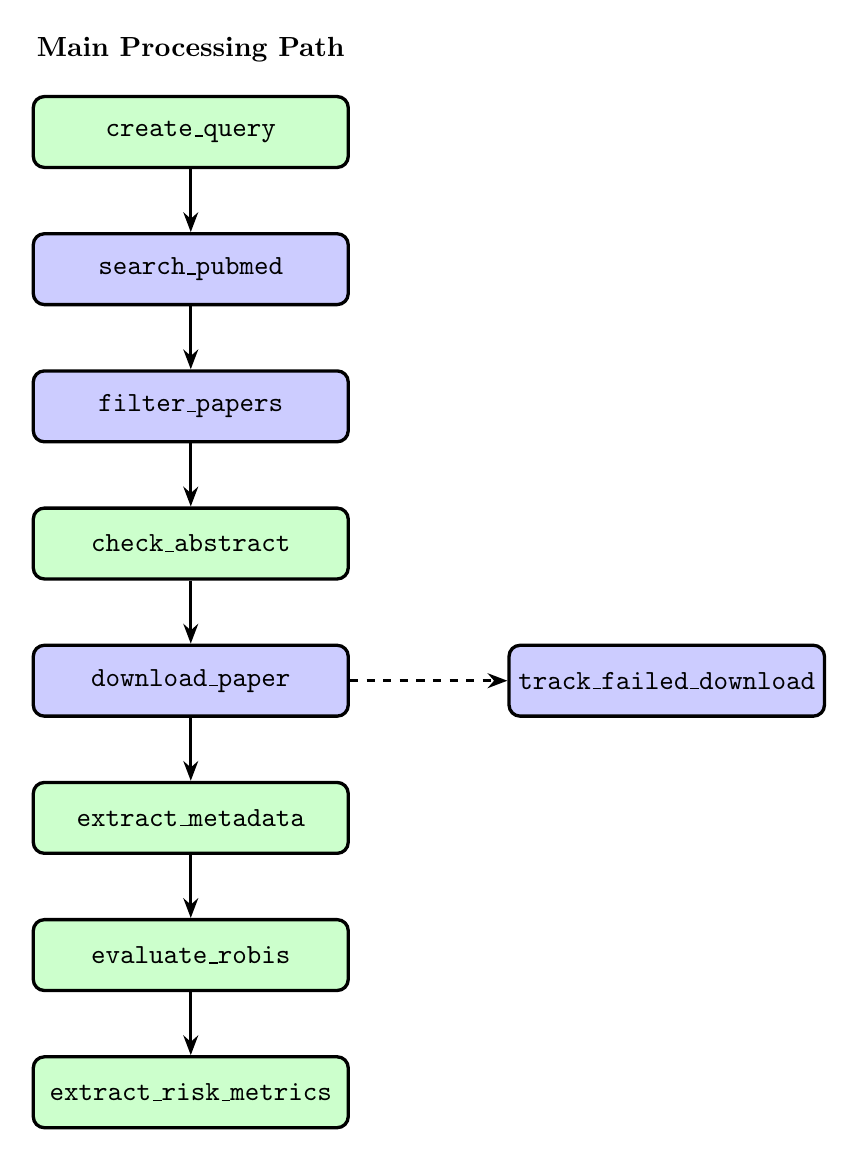
\begin{tikzpicture}[
    node distance=0.8cm,
    ai/.style={rectangle, rounded corners, minimum width=4cm, minimum height=0.9cm, text centered, draw=black, fill=green!20, very thick},
    tool/.style={rectangle, rounded corners, minimum width=4cm, minimum height=0.9cm, text centered, draw=black, fill=blue!20, very thick},
    arrow/.style={-{Stealth[length=2.5mm]}, very thick}
]

% Linear vertical flow
\node[text centered] (title) {\textbf{Main Processing Path}};
\node[ai, below=0.3cm of title] (cq) {\texttt{create\_query}};
\node[tool, below=of cq] (sp) {\texttt{search\_pubmed}};
\node[tool, below=of sp] (fp) {\texttt{filter\_papers}};
\node[ai, below=of fp] (ca) {\texttt{check\_abstract}};
\node[tool, below=of ca] (dp) {\texttt{download\_paper}};
\node[ai, below=of dp] (em) {\texttt{extract\_metadata}};
\node[ai, below=of em] (er) {\texttt{evaluate\_robis}};
\node[ai, below=of er] (ei) {\texttt{extract\_risk\_metrics}};

% Arrows
\draw [arrow] (cq) -- (sp);
\draw [arrow] (sp) -- (fp);
\draw [arrow] (fp) -- (ca);
\draw [arrow] (ca) -- (dp);
\draw [arrow] (dp) -- (em);
\draw [arrow] (em) -- (er);
\draw [arrow] (er) -- (ei);

% Side branch
\node[tool, right=2cm of dp] (tfd) {\texttt{track\_failed\_download}};
\draw [arrow, dashed] (dp) -- (tfd);

\end{tikzpicture}
\caption{Agent processing nodes in sequential order. Green = AI-powered nodes, Blue = tool/logic nodes. Dashed line shows alternative path for failed downloads.}
\label{fig:nodes}
\end{figure}

\subsection{Routing Logic}

The agent uses four conditional routing points to determine next actions based on current state:

\begin{table}[t]
\centering
\footnotesize
\begin{tabular}{|p{2.5cm}|p{3.5cm}|p{6.5cm}|}
\hline
\textbf{Routing Point} & \textbf{Condition} & \textbf{Next Action} \\
\hline\hline
After \texttt{check\_abstract} & Paper is relevant & Proceed to \texttt{download\_paper} \\
\cline{2-3}
 & Not relevant, more papers available & Return to \texttt{check\_abstract} (next paper) \\
\cline{2-3}
 & Not relevant, no papers left & Return to \texttt{create\_query} (new search) \\
\hline
After \texttt{download\_paper} & Download succeeded & Proceed to \texttt{extract\_metadata} \\
\cline{2-3}
 & Download failed & Go to \texttt{track\_failed\_download} \\
\hline
After \texttt{track\_failed\_download} & More papers available & Return to \texttt{check\_abstract} \\
\cline{2-3}
 & No papers left & Return to \texttt{create\_query} \\
\hline
After \texttt{extract\_risk\_metrics} & Target metrics reached & Terminate (END) \\
\cline{2-3}
 & Need more, papers available & Return to \texttt{check\_abstract} \\
\cline{2-3}
 & Need more, no papers left & Return to \texttt{create\_query} \\
\hline
\end{tabular}
\caption{Conditional routing logic at each decision point. The agent loops until collecting sufficient metrics or exhausting search space.}
\label{tab:routing}
\end{table}

\subsection{Workflow Description}

The complete workflow operates as follows: (1) The agent generates PubMed search queries adapted from previous attempts; (2) searches return up to 500 meta-analyses; (3) papers are filtered against already-checked DOIs; (4) abstracts are evaluated for relevance using LLM classification; (5) relevant papers are downloaded with fallback strategies; (6) successful PDFs undergo metadata extraction, ROBIS quality assessment, and risk metric extraction; (7) failed downloads are logged for manual processing; (8) the cycle continues until the target number of metrics is collected or search space is exhausted.

\printbibliography

\end{document}